\documentclass[11pt,a4paper]{article}

% == Packages ==============================================
\usepackage[utf8]{inputenc}
\usepackage[T1]{fontenc}
\usepackage{amsmath,amssymb}
\usepackage{graphicx}
\usepackage{booktabs}
\usepackage{multirow}
\usepackage{xcolor}
\usepackage{hyperref}
\usepackage[margin=1in]{geometry}
\usepackage{caption}
\usepackage{natbib}
\usepackage{microtype}
\usepackage{tikz}
\usetikzlibrary{positioning,arrows.meta,calc,shapes.geometric}

\hypersetup{colorlinks=true,linkcolor=blue!60!black,citecolor=blue!60!black,urlcolor=blue!60!black}

% == Macros ================================================
\newcommand{\laimark}{\textsc{Laimark}}

% ==========================================================
\title{\laimark{}: Gains and Structural Limits of Self-Generated Curricula\\in Reinforcement Learning from Verifiable Reward}

\author{Jes\'us Tabares Montilla\\
Independent Researcher\\
\texttt{jesus@tabares.eu}\\
\url{https://tabares.eu}}

\date{April 2026}

\begin{document}
\maketitle

% ==========================================================
\begin{abstract}
A language model can improve itself via reinforcement learning from verifiable reward if someone supplies the problems.
We ask what happens when the same model supplies them.

On HumanEval with Qwen3-8B, a pipeline that generates candidate programming problems and keeps the ones the base model solves inconsistently produces 33 usable problems.
GRPO on those alone raises pass@1 from 63.4\% to 76.8\%.
The same GRPO recipe on 664 curated problems from HumanEval and MBPP reaches 84.1\%; self-generation recovers 65\% of that gain on two orders of magnitude less training data.

Three limits cap the approach.
Iteration does not accumulate: a second GRPO round on problems calibrated against the first-round checkpoint converges back to it, because training on those problems raises the checkpoint's pass rate on them to 1.
A curriculum dominated by a single task type---84\% abduction in our experiment---drops pass@1 to 61.0\%, below the pre-training baseline, by shifting the output-format prior away from what HumanEval rewards.
At 32B parameters the learnability window closes entirely: the base model solves essentially every problem it can formulate with a verified reference solution, so calibration has nothing left to accept.

A per-problem inspection of the 8B checkpoint shows that eight of ten cases where the trained adapter beats its base are indentation fixes on code the base already writes correctly.
One case is a genuine reasoning gain.
GRPO at this scale teaches the model to format its answers for the evaluator; new reasoning is the minority component.
The same closed-loop structure that makes self-generation cost-free is what caps it.
\end{abstract}

% ==========================================================
\section{Introduction}
\label{sec:intro}

Reinforcement learning from verifiable reward (RLVR) has become the dominant post-training technique for language models on reasoning benchmarks.
\textsc{DeepSeek-R1}~\citep{deepseek2025r1} showed that Group Relative Policy Optimization (GRPO)~\citep{shao2024grpo} can elicit substantial reasoning capability from a pretrained base, provided each problem has an automatic evaluator: mathematical proofs, unit-tested programs, multiple-choice answers.
Every such system depends on the same input: a curated set of problems, written and verified by humans.
HumanEval~\citep{chen2021codex}, MBPP~\citep{austin2021mbpp}, GSM8K~\citep{cobbe2021training}, MATH.
The evaluators are cheap to run; the problems they evaluate are not free.

Self-generation is the obvious alternative.
Absolute Zero Reasoner (AZR)~\citep{zhao2025azr} trains proposer and solver networks on self-generated problems with verifiable answers and reports reasoning gains without curated training data.
The Darwin G{\"o}del Machine (DGM)~\citep{zhang2025dgm} takes a different angle: an LLM-driven agent edits its own Python source and keeps variants that improve a held-out score.
Both raise the same question.
If a model can generate its own problems and verify them, can it train on them and reach the performance of externally curated benchmarks?

We examine the question at a scale where the machinery is instrumentable: Qwen3-8B~\citep{qwen3} as the base model, HumanEval as the held-out evaluation.
The reference point is GRPO on curated problems: applied to Qwen3-8B with 664 problems from HumanEval and MBPP, GRPO raises pass@1 from 63.4\% to 84.1\% (official HuggingFace fp16 evaluator, +34 problems solved, 0 regressions).
The empirical question is what happens when the same base model is given only its own generations and a Python interpreter as evaluator.

\paragraph{What works.}
A generation-plus-calibration pipeline that keeps only problems the base model solves some of the time but not all of the time produces 33 usable problems from a pool of 1000 candidates.
GRPO on those 33 problems raises pass@1 from 63.4\% to 76.8\%.
That is 65\% of the 20.7-point improvement that the same training recipe extracts from 664 curated problems, at two orders of magnitude less training data.
A second finding cuts across the whole result: the number of rollouts per prompt in GRPO, \texttt{num\_generations}, matters more than the number of prompts at this data volume.
Moving \texttt{num\_generations} from 2 to 4 on identical data moves pass@1 by 6.7 points.
Within-batch gradient-signal contrast is what is scarce on small curricula, not prompts.

\paragraph{What does not.}
The approach fails to scale in three distinct ways, each with its own mechanism.
Iteration does not accumulate.
A second GRPO round trained on problems calibrated against the first-round checkpoint converges back to the checkpoint, because raising its pass rate on those problems to 1 is exactly what the training does.
Task-type imbalance destroys transfer.
A curriculum where 84\% of the calibrated problems are abduction-style---short scalar outputs---drops pass@1 on induction-style HumanEval to 61.0\%, below the pre-training baseline.
The adapter learns to emit short outputs and loses the indentation prior that induction needs.
Diversity in the curriculum regularizes; diversity concentrated in a single incompatible type is actively destructive.
Finally, moving from Qwen3-8B (63.4\% base) to Qwen3-32B (89.0\% base) collapses the learnability window: less than 1\% of problems the 32B model generates are solved sometimes-but-not-always by itself, and 0\% of the problems it labels ``hard'' pass calibration.
A generator-solver pair capable of producing well-formed verified problems is, by that same capability, able to solve them.

\paragraph{What the adapter actually learns.}
A per-problem inspection of the trained checkpoint separates format from reasoning.
Of 29 problems calibrated against the trained adapter, the adapter outperforms the base on ten.
Eight of those ten are formatting: the base writes code that would return the right answer if the interpreter accepted it, but places the body flush against the \texttt{def} line rather than indented, and the interpreter rejects the whole thing.
The adapter reliably inserts the leading whitespace.
One case is a genuine reasoning improvement: on \texttt{is\_valid\_date}, the base feeds the datetime format string through \texttt{re.fullmatch} and the \texttt{\%} characters break the match; the adapter skips the regex guard.
The remaining case is inconclusive on resampling.
The framing of RLVR at this scale as ``teaching the model to reason'' overstates what the adapter does.
``Teaching the model to present its output in the evaluator's expected format'' describes most of the effect.

\paragraph{The LAIMARK system.}
The experiments of this paper sit inside a larger closed-loop system we call LAIMARK (Local AI Metacognitive Agent with Recursive Knowledge).
LAIMARK has four components, all running on the same base model with no external agent, judge, or human-in-the-loop.

\begin{enumerate}
    \item \textbf{Prompt evolution}: an agent evolves system prompts against a held-out code-generation benchmark, producing the L2b prompt used throughout this paper (\S\ref{sec:background-l2}).
    \item \textbf{Weight update (GRPO)}: training a LoRA adapter via GRPO on verifiable-reward problems (this paper's main empirical object).
    \item \textbf{Self-refinement}: the weight-updated model re-enters the prompt-evolution phase and discovers an improved prompt for itself (\S\ref{sec:related}).
    \item \textbf{Self-generated curricula}: the weight-updated model generates the problems its own next GRPO round trains on (\S\ref{sec:main}--\ref{sec:limits}).
\end{enumerate}

Prior self-improvement systems operate on strict subsets.
DGM~\citep{zhang2025dgm} and its recursive extension Hyperagents~\citep{zhang2026hyperagents} run on component 1 at the agent-code level; they do not modify model weights.
DeepSeek-R1~\citep{deepseek2025r1} runs component 2 on curated external problems; it does not include prompts-as-data, self-refinement, or self-generation.
AZR~\citep{zhao2025azr} runs components 2 and 4 jointly; it does not include prompt evolution or self-refinement of prompts.
The composition of all four is what we mean by LAIMARK; this paper is the empirical study of components 2 and 4, including the structural limits their interaction exposes.
Figure~\ref{fig:loop} illustrates the full loop.

\paragraph{Contributions.}
\begin{enumerate}
    \item A closed-loop GRPO pipeline with no external problem source recovers 65\% of the gain available from 664 curated problems on HumanEval with Qwen3-8B (\S\ref{sec:main}).
    \item On small calibrated curricula, within-batch contrast (\texttt{num\_generations}) drives the result more than curriculum size; the precise mechanism---what fraction of training steps produce non-zero group advantage---is quantified in \S\ref{sec:main}.
    \item Three structural limits of the closed loop: iteration does not accumulate across rounds; calibrated curricula with a dominant task type destroy transfer; and the learnability window empties once the generator is strong enough to solve what it can propose (\S\ref{sec:limits}).
    \item A per-problem decomposition places most of GRPO's improvement at this scale in output formatting rather than in reasoning capability, qualifying a common claim about what RLVR teaches (\S\ref{sec:formatting}).
    \item LAIMARK composes prompt evolution, weight update, self-refinement, and self-generated curricula into a closed-loop system on a single base model; Figure~\ref{fig:loop} and \S\ref{sec:background-l2} differentiate it from DGM / Hyperagents (agent-level code only), DeepSeek-R1 (weights only, curated), and AZR (weights plus self-generation, no prompt evolution).
\end{enumerate}

\paragraph{Scope.}
This paper covers LAIMARK's components 2 and 4 empirically; components 1 and 3 appear as context.
Agent-level self-modification of the training code or reward function---the direction explored by the G{\"o}del Machine~\citep{schmidhuber2003godel} and by Hyperagents~\citep{zhang2026hyperagents}---is out of scope, as are signal sources outside the model's own output distribution (perception, physical environments, human feedback).
The structural limits reported here motivate both directions as follow-ups, discussed in \S\ref{sec:discussion}.
All reported pass@1 numbers use the official HuggingFace fp16 HumanEval evaluator.

% ----- Figure 1: Closed-loop LAIMARK system --------
\begin{figure}[t]
\centering
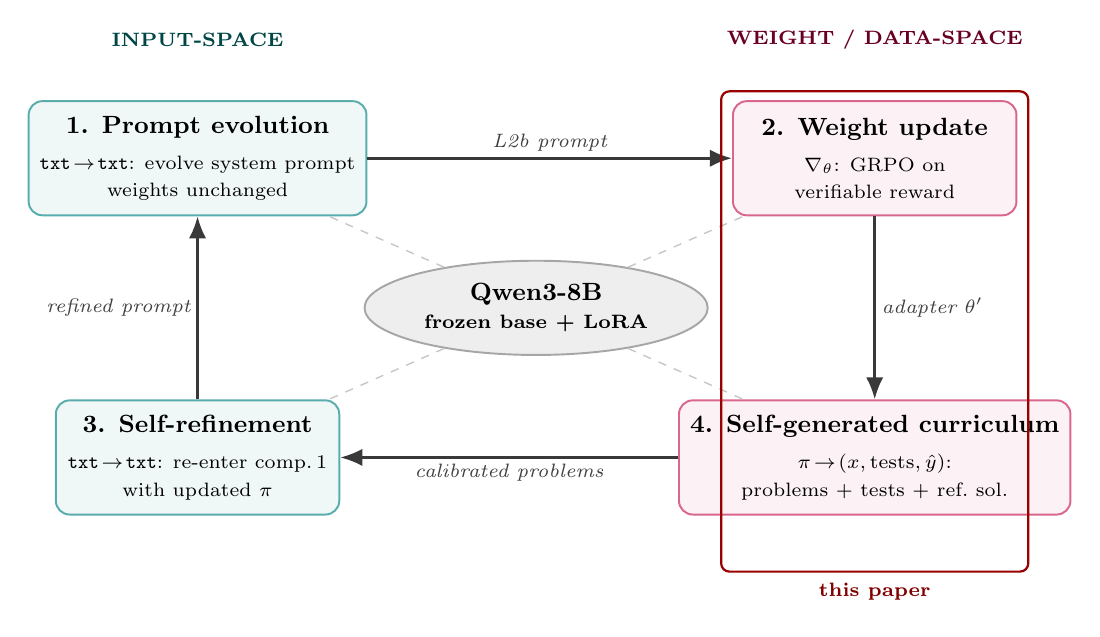
\begin{tikzpicture}[
    promptop/.style={rectangle, rounded corners=5pt,
                     draw=teal!65, fill=teal!6, line width=0.7pt,
                     align=center, minimum width=3.6cm, minimum height=1.45cm, font=\small,
                     inner sep=4pt},
    weightop/.style={rectangle, rounded corners=5pt,
                     draw=purple!60, fill=purple!5, line width=0.7pt,
                     align=center, minimum width=3.6cm, minimum height=1.45cm, font=\small,
                     inner sep=4pt},
    hub/.style={ellipse, draw=gray!70, fill=gray!13, line width=0.7pt,
                align=center, font=\small\bfseries, minimum width=3.1cm, minimum height=1.1cm},
    flow/.style={-{Latex[length=2.8mm, width=2.2mm]}, line width=1pt, draw=gray!45!black},
    uses/.style={dashed, draw=gray!45, line width=0.5pt},
    elab/.style={font=\scriptsize\itshape, text=gray!50!black, align=center,
                 inner sep=2pt, fill=white},
    tag/.style={font=\scriptsize\bfseries, text=gray!60!black, inner sep=1pt}
]

% --- central hub (the shared base model) ---
\node[hub] (hub) at (0,0) {Qwen3-8B\\[-1pt]\scriptsize frozen base + LoRA};

% --- four components arranged around the hub ---
\node[promptop] (prompt)  at (-4.3,  1.9)
    {\textbf{1. Prompt evolution}\\[2pt]
     \scriptsize $\mathtt{txt}\!\to\!\mathtt{txt}$: evolve system prompt\\[-1pt]
     \scriptsize weights unchanged};

\node[weightop] (weights) at ( 4.3,  1.9)
    {\textbf{2. Weight update}\\[2pt]
     \scriptsize $\nabla_\theta$: GRPO on\\[-1pt]
     \scriptsize verifiable reward};

\node[weightop] (selfgen) at ( 4.3, -1.9)
    {\textbf{4. Self-generated curriculum}\\[2pt]
     \scriptsize $\pi\!\to\!(x,\text{tests},\hat{y})$:\\[-1pt]
     \scriptsize problems + tests + ref.\ sol.};

\node[promptop] (refine)  at (-4.3, -1.9)
    {\textbf{3. Self-refinement}\\[2pt]
     \scriptsize $\mathtt{txt}\!\to\!\mathtt{txt}$: re-enter comp.\,1\\[-1pt]
     \scriptsize with updated $\pi$};

% --- dashed lines: each component reads/writes the shared model ---
\draw[uses] (hub) -- (prompt);
\draw[uses] (hub) -- (weights);
\draw[uses] (hub) -- (selfgen);
\draw[uses] (hub) -- (refine);

% --- solid flow arrows: the outer loop ---
\draw[flow] (prompt.east)   -- node[elab, above] {L2b prompt} (weights.west);
\draw[flow] (weights.south) -- node[elab, right] {adapter $\theta'$} (selfgen.north);
\draw[flow] (selfgen.west)  -- node[elab, below] {calibrated problems} (refine.east);
\draw[flow] (refine.north)  -- node[elab, left]  {refined prompt} (prompt.south);

% --- type legend top-right corner ---
\node[tag, text=teal!55!black] at (-4.3,  3.4) {INPUT-SPACE};
\node[tag, text=purple!55!black] at ( 4.3,  3.4) {WEIGHT / DATA-SPACE};

% --- scope bracket: this paper ---
\draw[thick, red!60!black, line width=0.8pt, rounded corners=3pt]
    ( 2.35, -3.35) rectangle ( 6.25,  2.75);
\node[font=\scriptsize\bfseries, text=red!50!black] at (4.3, -3.6) {this paper};

\end{tikzpicture}
\caption{The LAIMARK closed loop.
Four components, all running on the same base model (centre, dashed), with no external agent, judge, or human-in-the-loop.
Teal = \emph{input-space} operations (system prompts, weights unchanged); purple = \emph{weight or data-space} operations (LoRA update or problem synthesis).
The outer cycle shows the data flow of one full round.
This paper empirically studies components 2 and 4 (red box; \S\ref{sec:main}--\ref{sec:limits}) and summarises components 1 and 3 as context (\S\ref{sec:background-l2}, \S\ref{sec:related}).
Prior work covers strict subsets along this axis: DGM and Hyperagents~\citep{zhang2025dgm,zhang2026hyperagents} modify agent-level code (a broader notion of component 1) without touching weights; DeepSeek-R1~\citep{deepseek2025r1} runs component 2 on curated external problems; AZR~\citep{zhao2025azr} runs components 2 and 4 jointly without a prompt-evolution phase.}
\label{fig:loop}
\end{figure}

% ==========================================================
\section{Background}
\label{sec:background}

\paragraph{GRPO.}
Group Relative Policy Optimization~\citep{shao2024grpo} updates a policy $\pi_\theta$ using groups of $G$ rollouts per prompt.
Given prompt $x$, the policy samples completions $\{y_k\}_{k=1}^G$, each receives reward $r_k$, and the advantage for each rollout is normalized within the group:
\begin{equation}
    A_k = \frac{r_k - \mathrm{mean}(\{r_i\})}{\mathrm{std}(\{r_i\}) + \epsilon}.
    \label{eq:grpo-adv}
\end{equation}
The gradient update is $\nabla_\theta \log \pi_\theta(y_k \mid x) \cdot A_k$, regularized by a KL term to a reference policy.
When all $r_k$ are equal, $A_k$ is zero for every rollout in the group, and a prompt on which the policy always passes or always fails contributes nothing to training.

\paragraph{The learnability window.}
Useful training data for GRPO is not what the policy cannot solve; it is what the policy solves \emph{inconsistently}.
Let $p(x) = \Pr[r(y) = 1 \mid y \sim \pi_\theta(\cdot \mid x)]$ be the pass rate of the current policy on prompt $x$.
Prompts with $p(x) \in \{0, 1\}$ produce no gradient; prompts with $p(x) \in (0, 1)$ do, with the signal peaking near $p(x) = 0.5$.
We call prompts with $p(x) \in [\delta, 1-\delta]$ the \emph{learnability window} at threshold $\delta$.
Calibration, in our pipeline, is the operation that estimates $p(x)$ by sampling and keeps only prompts inside this window.

\paragraph{Closed-loop self-evolution.}
A training loop is \emph{closed} when the same base model serves as problem generator, candidate-solution generator, and source of the reference solution from which unit tests are checked.
The evaluator---the Python interpreter---remains external and deterministic, but every object it evaluates originates from the model.
Under this constraint, the model's competence bounds both (a) the complexity of problems it can formulate with a correct reference solution, and (b) the prompts for which rollouts produce reward variance.
Section~\ref{sec:limits-scale} shows these two bounds collide for strong enough models: a generator capable of producing well-formed verified problems is also capable of solving them, and the learnability window closes.

\paragraph{Prior work on self-generation.}
AZR~\citep{zhao2025azr} trains a proposer and a solver in the same RL loop, with the proposer rewarded for producing problems the solver finds difficult and the solver rewarded for solving them.
The two networks share parameters in early experiments and diverge in later ones.
AZR reports sustained improvement on reasoning benchmarks without externally curated training problems.
Three differences matter for interpreting our results: (i) we do not co-evolve proposer and solver---generation and calibration are offline stages with separate checkpoints---(ii) we operate at 8B and 32B parameters rather than frontier scale, and (iii) we test iteration across training rounds and find it does not accumulate (\S\ref{sec:limits-iter}), a regime we do not see examined directly in AZR.
DGM~\citep{zhang2025dgm} addresses a different question: an agent modifies its own Python source code and is retained if a held-out benchmark improves.
Its extension Hyperagents~\citep{zhang2026hyperagents} applies the same agent-level modification recursively.
Both are about agent-level self-modification of training logic; we are about training a model on self-generated data, holding training logic fixed.
Their relationship is discussed in \S\ref{sec:related}.

\subsection{The L2 taxonomy and the L2b prompt}
\label{sec:background-l2}

The experiments throughout this paper use a specific system prompt rather than a generic one.
That prompt is the endpoint of a prior phase of LAIMARK which evolved system prompts against a code-generation benchmark while holding weights fixed; the classification we summarize here is a side effect of that run, and it frames how we read what GRPO can and cannot add on top.

A prompt-evolution agent that scores system prompts by a held-out pass@1 converges to three qualitatively distinct kinds of high-scoring prompts.

\begin{description}
    \item[L1 (literal).] The prompt embeds a solution to a specific problem in the evaluation subset (``the \texttt{is\_happy} function returns \texttt{True} if ...'').
    The score on that problem spikes; scores on disjoint test problems are erratic or regress.
    L1 is the canonical reward-hacking failure: a cheat, not an improvement.
    \item[L2a (conceptual).] The prompt names the class the target problem belongs to (``use dynamic programming to maintain a running sum'').
    Scores improve modestly and generalize across problems sharing that concept but not across concepts.
    \item[L2b (operational).] The prompt describes \emph{procedure}: how to decompose the output, how to iterate, which invariants to maintain, what to verify before returning.
    Scores improve substantially and generalize across problems regardless of whether they share a specific concept.
\end{description}

L2b is the class that produces the largest gains on an open coding evaluation in our prompt-evolution runs.
It is also the class the agent converges to without being directed: L2b prompts dominate the fitness landscape when the only signal is pass@1 on a held-out subset.
A variant of this effect appears independently in the prompts that Qwen3-8B generates when L2b is its own system message versus when it is not: the L2b-prompted model writes more procedurally structured code.

The L2b prompt used throughout this paper instructs the model to (i) initialize result containers explicitly, (ii) iterate with explicit type-checking, (iii) maintain and update accumulators systematically, and (iv) verify outputs match expected types and constraints.
The prompt is a frozen output of a prior evolution run; we do not claim to be rediscovering it here.

L2b does not add reasoning capability.
It adds an output-distribution shift that biases the model toward procedural, step-by-step code, and its effect size depends on how underrepresented such code is in the model's default output distribution.
Qwen3-32B, which already writes more procedural code by default, loses 1.2 pass@1 points under L2b (\S\ref{sec:limits-scale}).
The same shift that helps the 8B model hurts the 32B model, which is the first instance of a pattern recurring through the rest of the paper: at this scale, RLVR and its prompt-level counterparts shape output distributions more than they grow capability (\S\ref{sec:formatting}).

% ==========================================================
\section{Self-Generation and Calibration Pipeline}
\label{sec:method}

Figure~\ref{fig:pipeline} summarizes the full pipeline for one training round.
The subsections that follow describe each stage.

% ----- Figure 2: Pipeline -------------------------
\begin{figure}[t]
\centering
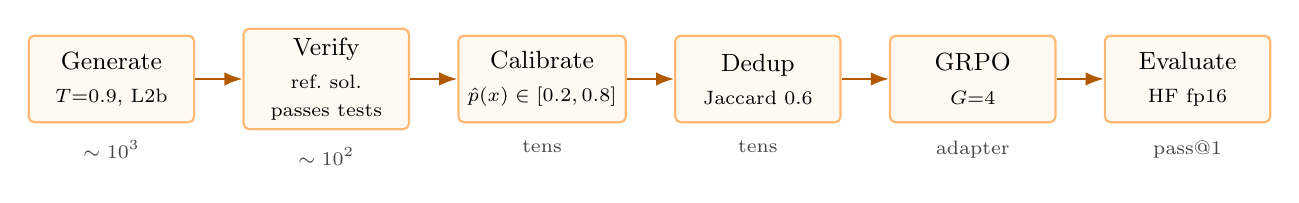
\begin{tikzpicture}[
    stage/.style={rectangle, rounded corners=2pt, draw=orange!55, fill=orange!5, thick,
                  align=center, minimum width=2.1cm, minimum height=1.1cm, font=\small},
    arrow/.style={-{Latex[length=2.3mm]}, thick, draw=orange!70!black},
    clabel/.style={font=\scriptsize, text=gray!55!black, align=center}
]

\node[stage]                        (gen)    {Generate\\[1pt] \scriptsize $T{=}0.9$, L2b};
\node[stage, right=0.6cm of gen]    (verify) {Verify\\[1pt] \scriptsize ref.\ sol.\\[-1pt] \scriptsize passes tests};
\node[stage, right=0.6cm of verify] (calib)  {Calibrate\\[1pt] \scriptsize $\hat{p}(x)\in[0.2,0.8]$};
\node[stage, right=0.6cm of calib]  (dedup)  {Dedup\\[1pt] \scriptsize Jaccard 0.6};
\node[stage, right=0.6cm of dedup]  (grpo)   {GRPO\\[1pt] \scriptsize $G{=}4$};
\node[stage, right=0.6cm of grpo]   (eval)   {Evaluate\\[1pt] \scriptsize HF fp16};

\draw[arrow] (gen) -- (verify);
\draw[arrow] (verify) -- (calib);
\draw[arrow] (calib) -- (dedup);
\draw[arrow] (dedup) -- (grpo);
\draw[arrow] (grpo)  -- (eval);

\node[below=0.10cm of gen,    clabel] {$\sim 10^3$};
\node[below=0.10cm of verify, clabel] {$\sim 10^2$};
\node[below=0.10cm of calib,  clabel] {tens};
\node[below=0.10cm of dedup,  clabel] {tens};
\node[below=0.10cm of grpo,   clabel] {adapter};
\node[below=0.10cm of eval,   clabel] {pass@1};

\end{tikzpicture}
\caption{Self-generation and training pipeline for one round.
Numbers under each stage are order-of-magnitude counts at Qwen3-8B.
At Qwen3-32B (\S\ref{sec:limits-scale}), the calibration stage accepts less than 1\% of candidates and the pipeline terminates for lack of training data.}
\label{fig:pipeline}
\end{figure}

\subsection{Base model and adapter}
\label{sec:method-model}

The base model is Qwen3-8B~\citep{qwen3}; the 32B experiments in \S\ref{sec:limits-scale} use Qwen3-32B.
Training adapts a LoRA module~\citep{hu2022lora} (rank 16, $\alpha = 32$, dropout 0.05) on the attention query and value projections ($q_{\text{proj}}$, $v_{\text{proj}}$).
Base weights stay frozen.
At evaluation the adapter is merged into the base and the merged model is run in fp16 with the official HumanEval harness.
One property of this setup is worth stating early: the adapter capacity is small---one rank-16 update per attention layer, on two of four projections---enough to shift output distributions reliably but far from enough to rewrite arbitrary base-model knowledge.
Section~\ref{sec:formatting} returns to the consequences.

\subsection{Problem generation}
\label{sec:method-gen}

A candidate problem is a triple: function signature with docstring, unit tests as Python \texttt{assert} statements, and a reference solution.
The generation prompt requests all three parts in a fixed format, paired with a topic drawn from twenty general-purpose categories---\emph{string manipulation}, \emph{number theory}, \emph{dictionary operations}, \emph{bit manipulation}, and similar---and a difficulty label (\emph{hard} or \emph{very hard}).
Sampling uses temperature 0.9 for diversity.
Responses are parsed by fixed markers (\texttt{FUNCTION:}, \texttt{TESTS:}, \texttt{SOLUTION:}); malformed responses are discarded.

\subsection{Verification}

A candidate survives verification if its reference solution, executed against its own unit tests in a Python subprocess with a five-second timeout, produces no assertion failure and no uncaught exception.
This stage filters candidates with broken code, incorrect reference solutions, or non-terminating control flow.
It does not yet test the base policy against the problem---it only checks the problem is internally consistent.

\subsection{Calibration}
\label{sec:method-calib}

A verified problem enters the training curriculum only if its pass rate under the base policy lies inside the learnability window.
We estimate $p(x)$ by drawing $K = 8$ completions with the L2b system prompt (component 1 of the LAIMARK system, described in \S\ref{sec:background-l2}) and counting completions that pass all unit tests.
Candidates with $\hat{p}(x) \in [0.2, 0.8]$ are retained; consistently solved or consistently failed candidates are discarded.

Calibration is the bottleneck of the pipeline.
On Qwen3-8B, roughly one verified candidate in ten survives it.
On Qwen3-32B the ratio collapses to the order of 1\% (\S\ref{sec:limits-scale}).

Surviving problems are deduplicated by function-name exact match and by Jaccard similarity over word trigrams on the docstring (threshold 0.6).

\subsection{GRPO training}
\label{sec:method-grpo}

Training uses the TRL implementation of GRPO on top of the frozen base and the LoRA adapter from \S\ref{sec:method-model}.
Each prompt produces $G$ rollouts per step; the reward of a rollout is 1 if the model's completion passes all unit tests of the corresponding problem (under the same subprocess harness used during verification) and 0 otherwise.
Default settings are $G = 4$, learning rate $5 \times 10^{-6}$ with cosine decay and $10\%$ warmup, per-device batch size 4, two epochs, maximum completion length 1024 tokens, and AdamW.
All calibrated problems are equally weighted by default; a variant weighting each problem by $1 - |2\hat{p}(x) - 1|$ (maximum weight at $\hat{p} = 0.5$) yielded indistinguishable results and is not used in the reported numbers.

$G$ is the hyperparameter whose effect dominates the results at small data volumes.
Section~\ref{sec:main} reports that shifting from $G = 2$ to $G = 4$ on the same 33-problem selfgen curriculum moves pass@1 from 70.1\% to 76.8\%, a gain comparable to adding several hundred curated problems.

\subsection{Evaluation protocol}
\label{sec:method-eval}

All pass@1 numbers in this paper use the official HumanEval test set with the standard HuggingFace fp16 evaluator, greedy decoding (temperature 0), and one sample per problem.
Self-generated curricula never contain HumanEval problems: we explicitly check the function name and docstring trigram similarity against the HumanEval test set and reject candidates that overlap.
The curated-benchmark baseline uses HumanEval and MBPP~\citep{austin2021mbpp} training splits, with problem identifiers verified not to intersect the HumanEval test set.\footnote{%
The distinction between HumanEval train and test splits is not inherent to HumanEval, which is a test-only benchmark.
We treat problems the base model has seen during pretraining as implicitly available and use MBPP as the main source of external problems.
The 664-problem figure refers to HumanEval + MBPP combined after deduplication.}

Every other evaluation system we considered---Ollama-based evaluation in particular---disagrees with the HF fp16 harness by several points due to quantization and prompt-template differences.
We do not mix them, and we flag this as the dominant source of apparent disagreement between our numbers and informal reports in the community.

% ==========================================================
\section{Main Result}
\label{sec:main}

We compare three training configurations against the Qwen3-8B base, all evaluated with the official HumanEval fp16 harness (\S\ref{sec:method-eval}).

\begin{description}
    \item[Base.] Qwen3-8B, no adapter. 63.4\% pass@1.
    \item[Curated.] GRPO on hundreds of problems drawn from HumanEval and MBPP training splits ($G = 4$, otherwise matching \S\ref{sec:method-grpo}). 84.1\% pass@1.
    \item[Selfgen.] GRPO on tens of self-generated, calibrated problems, zero external benchmarks. Two variants: $G = 2$ (\emph{v1}) and $G = 4$ (\emph{v2}).
\end{description}

Table~\ref{tab:main} reports the full comparison.

\begin{table}[ht]
\centering
\caption{HumanEval pass@1 for GRPO on curated external problems versus self-generated calibrated problems on Qwen3-8B. ``Gain captured'' is the fraction of the curated-GRPO gain (+20.7 pts) recovered with zero external problems.}
\label{tab:main}
\begin{tabular}{lcccc}
\toprule
Configuration & External problems & $G$ & Pass@1 & Gain captured \\
\midrule
Base & --- & --- & 63.4\% & --- \\
Selfgen v1 & 0 & 2 & 70.1\% & 32\% \\
Selfgen v2 & 0 & 4 & \textbf{76.8\%} & \textbf{65\%} \\
Curated (HE+MBPP) & hundreds & 4 & 84.1\% & 100\% \\
\bottomrule
\end{tabular}
\end{table}

Selfgen v2 recovers roughly two-thirds of the curated-benchmark improvement using an amount of training data two orders of magnitude smaller---and none of it external.
This is the paper's positive result: a closed loop with nothing outside the model and a Python interpreter can reach 76.8\% pass@1 from a 63.4\% base.

\paragraph{Per-problem comparison against the base.}
Selfgen v2 solves 126 of the 164 HumanEval problems versus 104 for the base, a net gain of +22.
The curated GRPO, measured on the same split and harness, produces +34 problems solved and zero regressions against the base, accounting for the rest of the gap in Table~\ref{tab:main}.
Both adapters move the model in the same direction; selfgen v2 has lower coverage rather than different behavior, a distinction \S\ref{sec:formatting} makes quantitative.

\paragraph{Why contrast matters more than volume.}
The difference between selfgen v1 and v2 is the GRPO group size $G$: v1 uses $G = 2$, v2 uses $G = 4$, on identical data.
Within-batch advantage (Eq.~\ref{eq:grpo-adv}) is zero whenever all $G$ rollouts of a prompt receive the same reward.
At the training pass rates we observe ($\hat{p}(x) \approx 0.53$ mean across calibrated problems), moving from $G = 2$ to $G = 4$ changes the expected fraction of training steps with non-zero gradient from roughly $2\hat{p}(1-\hat{p}) \approx 0.50$ to $1 - \hat{p}^4 - (1-\hat{p})^4 \approx 0.88$.
Empirically, the fraction of non-degenerate training steps went from 30\% under $G=2$ to 80\% under $G=4$.
The 6.7-point gap between v1 and v2 is substantially explained by this factor alone.

A practical reading: at small curriculum sizes---tens of problems, not hundreds---$G$ has more leverage than adding more problems.
Doubling $G$ roughly halves the fraction of wasted training steps on a calibrated curriculum and, in our runs, contributes as much pass@1 gain as a substantial additional amount of curated data would.
This does not suggest that arbitrary $G$ helps: the rollouts share the same prompt, and the computation cost scales linearly in $G$.
The point is that \emph{calibration plus high $G$ is a complete substitute for curated-dataset volume in this regime}, and the two are not independent design choices.

% ==========================================================
\section{Where Self-Generated Curricula Fail}
\label{sec:limits}

The positive result of \S\ref{sec:main} might suggest a recipe: iterate the loop, diversify the curriculum, or scale the base model to push pass@1 higher.
We tried all three.
Each fails, in a different way and for a different structural reason.

\subsection{Iteration Does Not Accumulate}
\label{sec:limits-iter}

Starting from the v2 checkpoint, we ran the full pipeline a second time: generate problems with v2, verify them, calibrate against v2 (rather than against the base, as in the first round), and train GRPO on the survivors.
Two configurations were tested.

\begin{itemize}
    \item \textbf{Iter-2a} trains a fresh LoRA adapter on the base model using problems calibrated against v2. Pass@1: 65.2\%.
    \item \textbf{Iter-2b} merges v2's adapter into the base and trains a new LoRA on top, using the same problems. Pass@1: 76.8\%.
\end{itemize}

Both are at or below v2's own 76.8\%.
Iter-2a is worse because calibration mismatched the training policy: problems sitting in v2's learnability window do not sit in the base's, so most of them land outside $[0.2, 0.8]$ for the base and produce little gradient.
Iter-2b corrects this---it calibrates against the same checkpoint it trains from---and converges to exactly v2's pass@1, recovering the predecessor without improving on it.

The mechanism is the one the pipeline invites.
Calibration selects problems where $\hat{p}_{v2}(x) \in [0.2, 0.8]$.
Training on those problems raises $p_{v2}(x)$ toward 1.
The resulting checkpoint dominates the curriculum that was built for it.
For iteration to advance genuinely, v2 would need to generate problems that it cannot yet solve consistently \emph{and} produce a correct reference solution for them.
The pipeline requires both, and v2's competence bounds both.

We also measured the survival ratio of v2-generated problems through verification plus calibration against v2.
A pool of 696 candidates produced 24 problems that v2 verified and that fell in v2's learnability window---roughly 3.4\% survival.
A second generation pass, with v2 as generator, produced 1.7\% survival against the same criterion.
The learnability window is not just hard to hit on iteration; it is shrinking.

\subsection{Task-Type Imbalance Destroys Transfer}
\label{sec:limits-type}

If iteration does not advance, diversity might.
A natural next step: expand the curriculum beyond induction-style problems (``given the function, write its body'') to include deduction (``given inputs, predict outputs'') and abduction (``given input-output examples, recover the function'').
This is the triad used by AZR~\citep{zhao2025azr}.
We ran two rounds with different calibration regimes.

\paragraph{Round 0: diversity without calibration.}
The curriculum mixes 28 induction problems calibrated against v2, plus 84 deduction and 84 abduction problems left uncalibrated (Table~\ref{tab:r0r1}).
Of 196 prompts, calibration touches 14\%.
Training produces 80.5\% pass@1---a further +3.7 points over v2.

Why this works, in spite of most of the curriculum being uncalibrated: the uncalibrated deduction and abduction samples concentrate in the saturated regions ($r = 1$ always, or $r = 0$ always), where GRPO's group advantage is zero.
Approximately 10.8\% of training steps produced non-trivial gradient, and nearly all of that came from the 28 calibrated induction problems.
The non-induction problems acted as diverse noise that did not interfere with the induction signal.

\paragraph{Round 1: diversity with calibration.}
Following the Round-0 procedure, we calibrated every problem in a fresh pool against the Round-0 adapter and trained from it.
Calibration retains a 143-problem curriculum: 7 induction, 16 deduction, 120 abduction (Table~\ref{tab:r0r1}).
Training produces 61.0\% pass@1---below the pre-training baseline of 63.4\%.

\begin{table}[ht]
\centering
\caption{Curriculum composition for the two rounds of the task-type interference experiment. Round 1 pushes calibration coverage to 100\% and collapses to a task-type distribution dominated by abduction.}
\label{tab:r0r1}
\begin{tabular}{lcccccc}
\toprule
 & \multicolumn{3}{c}{Problems} & \multicolumn{1}{c}{Calibrated} & Useful & \multirow{2}{*}{Pass@1} \\
\cmidrule(lr){2-4}
Round & Induction & Deduction & Abduction & coverage & steps & \\
\midrule
R0 & 28 & 84 & 84 & 14\% & $\sim$11\% & \textbf{80.5\%} \\
R1 & 7 & 16 & 120 & 100\% & $\sim$60\% & 61.0\% \\
\bottomrule
\end{tabular}
\end{table}

Calibration does what calibration is supposed to do: raises the fraction of training steps with useful gradient from roughly 11\% to roughly 60\%.
But 84\% of the calibrated problems are abduction-style.
Abduction rewards short, scalar outputs (``the function is \texttt{lambda x: x + 2}''); induction rewards long, indented code blocks.
Training preferentially on short-output gradients teaches the model to emit short outputs.
When the test benchmark is induction-style (HumanEval), the policy has been shifted toward a format that does not apply.

An explicit measurement: of the 33 problems Round 1 loses relative to Round 0, 23 are Python indentation errors.
The adapter still produces code that is logically correct in many cases, but misformatted in a way that the interpreter rejects.
The regression is not about reasoning capability; it is about which format prior the training signal reinforces.

The point generalizes beyond our three task types.
Learnability-based calibration has no mechanism for controlling output-format distribution, and any curriculum whose calibrated majority has an output format that conflicts with the evaluation format will degrade evaluation performance---even when the curriculum's calibration is, by the usual metric, excellent.

\subsection{Inapplicability at Scale}
\label{sec:limits-scale}

The natural last move: use a larger base model.
We repeated the setup with Qwen3-32B in place of Qwen3-8B, keeping everything else fixed except the prompt format: Qwen3-32B's output distribution is poorly aligned with the ``body-only'' HumanEval prompt used for the 8B experiments, so we switched to a ``full-function'' format in which the model returns a complete function rather than a completion to an existing one.
The effect of the format change is itself informative and we return to it in \S\ref{sec:formatting}.

Table~\ref{tab:scale} compares base performance.
Qwen3-32B's pass@1 without any training is 89.0\%---higher than anything Qwen3-8B achieves after GRPO on hundreds of curated problems (84.1\%).
Applying the L2b system prompt that improved Qwen3-8B by several points (63.4\% $\to$ 66.9\% in a quick comparison) \emph{degrades} Qwen3-32B by 1.2 points.
L2b, in retrospect, is a prompt that compensates for specific Qwen3-8B failure modes that Qwen3-32B does not share.

\begin{table}[ht]
\centering
\caption{Base pass@1 for Qwen3-8B and Qwen3-32B. Full-function format for 32B reflects a format change; the 83-point difference between body-only (6.1\%) and full-function (89.0\%) for 32B quantifies how much output formatting accounts for.}
\label{tab:scale}
\begin{tabular}{lccc}
\toprule
Model & Prompt & Format & Pass@1 \\
\midrule
Qwen3-8B & L2b & body-only & 63.4\% \\
Qwen3-32B & generic & body-only & 6.1\% \\
Qwen3-32B & generic & full-function & \textbf{89.0\%} \\
Qwen3-32B & L2b & full-function & 87.8\% \\
\bottomrule
\end{tabular}
\end{table}

The structural question for the paper is what happens when a 32B generator proposes its own problems.
We ran the generation and calibration pipeline with Qwen3-32B as both proposer and calibration oracle.
Two pools (Table~\ref{tab:scale-selfgen}): one of 236 medium-difficulty candidates (reused from the 8B-generated pool of 2500, verified to parse for 32B) and a fresh pool of 10 hard candidates generated by the 32B model itself.
Acceptance rate of the medium pool: 0.85\%.
Acceptance rate of the hard pool: 0\%.

\begin{table}[ht]
\centering
\caption{Calibration acceptance rate for Qwen3-32B on two self-generated pools. The learnability window is empty at 32B.}
\label{tab:scale-selfgen}
\begin{tabular}{lccc}
\toprule
Pool & Generator & Candidates & Accepted \\
\midrule
Medium (verified) & Qwen3-8B & 236 & 2 (0.85\%) \\
Hard (verified) & Qwen3-32B & 10 & 0 (0.0\%) \\
\bottomrule
\end{tabular}
\end{table}

The mechanism is direct: calibration requires $\hat{p}(x) \in [0.2, 0.8]$, and 32B's $\hat{p}(x)$ sits at or near 1 on nearly every problem it can formulate with a verified reference solution.
A generator capable of producing well-formed problems \emph{with correct reference solutions} is, by that very capability, able to solve the problems it produces.
The learnability window is not a difficulty-of-problem measure; it is a pass-rate measure under the target policy.
When the generator and the target policy are the same model, and the generator's competence has grown, the window closes.

We know of no prior reporting of this collapse.
AZR and DeepSeek-R1 apply self-generation at scales where the solver still fails sometimes on problems the proposer can formulate; the regime where the two capabilities become coextensive has not, to our knowledge, been isolated.
The implication is not that self-generation breaks down somewhere between 8B and 32B specifically, but that any self-generation scheme relying on a learnability-window filter has a capability ceiling that is structurally below the generator's own competence.

% ==========================================================
\section{What GRPO Teaches: Formatting vs.\ Capability}
\label{sec:formatting}

A 13-point improvement in pass@1 after GRPO invites a natural interpretation: the model has learned to reason better.
A problem-level comparison complicates that reading.

\paragraph{Setup.}
We took 29 problems calibrated against v2 (23 from the original generated pool, 6 generated by v2 itself), sampled $K = 8$ completions from the base model on each, and compared the resulting pass rate to v2's pass rate on the same problems.
The comparison is conservative in two directions.
First, these problems were selected to sit in v2's learnability window, so they favor v2 by construction.
Second, we are comparing aggregate pass rates, not outputs token by token, so the comparison captures effects on reward but nothing finer.

\paragraph{Results.}
Table~\ref{tab:format-capability} summarizes the 29-problem breakdown.

\begin{table}[ht]
\centering
\caption{Problem-level comparison of base vs.\ v2 on 29 problems calibrated against v2 ($K = 8$ per problem).}
\label{tab:format-capability}
\begin{tabular}{lrr}
\toprule
Outcome & Problems & Fraction \\
\midrule
v2 pass rate $>$ base pass rate & 10 & 34\% \\
v2 pass rate $\approx$ base pass rate ($|\Delta| \leq 1/8$) & 18 & 62\% \\
v2 pass rate $<$ base pass rate & 1 & 3\% \\
\bottomrule
\end{tabular}
\end{table}

On 62\% of calibrated problems, base and v2 are indistinguishable.
The asymmetry between v2-wins (34\%) and base-wins (3\%) is real and accounts for the aggregate pass@1 gap, but already suggests that v2 is not strictly stronger on calibrated problems---it simply fails less often on a fraction of them.

\paragraph{Decomposition of the 10 v2-wins.}
We inspected the completions base and v2 produce on each of the ten problems where v2 improves (Table~\ref{tab:format-breakdown}).

\begin{table}[ht]
\centering
\caption{Mechanism behind each v2-win, from inspection of completions. ``Format'' indicates that the base model produces logically correct code that the interpreter rejects due to indentation or surrounding whitespace; v2's gain is that it emits correctly indented code. ``Logic'' indicates that v2's completion is meaningfully different, not a formatting variant. ``Inconclusive'' indicates that v2's advantage does not hold up under re-sampling.}
\label{tab:format-breakdown}
\begin{tabular}{lc}
\toprule
Mechanism & Problems \\
\midrule
Formatting (correct logic, broken indentation in base) & 8 \\
Logic (base-model failure mode absent in v2) & 1 \\
Inconclusive on re-sampling & 1 \\
\bottomrule
\end{tabular}
\end{table}

Eight of the ten v2-wins are cases where the base model produces code that would compute the right answer if the interpreter accepted it.
The base emits, for example, \texttt{def multiply\_matrix\_scalar(matrix, scalar):\textbackslash nreturn [[x * scalar for x in row] for row in matrix]}---a correct one-liner with the body placed flush against the \texttt{def} line rather than indented.
v2 reliably inserts the leading whitespace.
The training-time reward signal---pass/fail from the interpreter---is sufficient to teach the emission of indentation, not more, in eight of ten cases.

\paragraph{The one genuine logic improvement.}
On \texttt{is\_valid\_date}, which asks for a function that validates a date string against a format string, the base model consistently calls \texttt{re.fullmatch(format\_str, date\_str)} before passing the pair to \texttt{datetime.strptime}, treating \texttt{"\%Y-\%m-\%d"} as a regular expression.
The \texttt{\%} characters are not valid regex; the validation fails for correctly-formatted dates; three of four base samples fail for this reason.
v2 skips the regex guard and passes directly to \texttt{strptime}, which accepts the format string correctly.
This is not a formatting fix.
The v2 adapter has---on this problem---absorbed a generalization that \texttt{\%}-prefixed format strings are datetime format specifiers and not regex.

\paragraph{Reading the decomposition.}
We read these numbers as a ceiling on the capability-learning hypothesis for RLVR at this scale and with this adapter capacity.
GRPO reliably teaches the model to present its answer in the format the evaluator rewards.
It can also, at a lower rate, propagate small reasoning improvements back into the adapter---the \texttt{is\_valid\_date} case is real, and we do not see a corresponding failure mode in v2.
But at LoRA rank 16 on two attention projections, the adapter has far more capacity to reshape output distributions than to rewrite knowledge, and most of what it learns reflects this ratio.

The scale experiments of \S\ref{sec:limits-scale} are consistent.
Qwen3-32B's pass@1 jumps from 6.1\% to 89.0\% when the prompt format is changed from ``body-only'' to ``full-function''---83 points of pass@1 attributable entirely to where the model's output is expected to appear.
Most of GRPO's work on Qwen3-8B is teaching the model a format convention that Qwen3-32B adopts without training, given a prompt that asks for it.
This does not make the 8B training pointless---the model does improve on some problems it previously failed for non-format reasons---but the ``GRPO teaches reasoning'' framing is at best a secondary component.

% ==========================================================
\section{Related Work}
\label{sec:related}

\paragraph{RLVR on curated benchmarks.}
DeepSeek-R1~\citep{deepseek2025r1} established the recipe this paper operates within: take a pretrained base model, apply GRPO~\citep{shao2024grpo} with automatic verifiers on mathematical and coding problems, obtain a model that generalizes beyond the training distribution.
DeepSeek-R1 was trained at frontier scale with many orders of magnitude more compute than any of our experiments; our contribution is not at that axis.
What we add is a controlled study of what happens when the curated curriculum is removed and replaced with the model's own generations, and a documentation of three structural limits of that substitution that the frontier-scale work has not been positioned to isolate.

\paragraph{Self-generation for reasoning.}
AZR~\citep{zhao2025azr} is the closest prior work.
A single model alternates between proposing problems (scored by a measure of difficulty for the solver) and solving them (scored by the proposer's verifier), in a shared-weight co-evolutionary loop.
AZR reports sustained improvement across rounds and across task types (deduction, abduction, induction), with no curated problems and verifiable rewards throughout.
Our results overlap AZR's in the positive finding that self-generation with verifiable reward produces real improvement without curated problems.
They diverge on two points.
First, we find that iteration across rounds with offline calibration does not accumulate (\S\ref{sec:limits-iter}); AZR does not, to our reading, report the pass@1 of the solver after full re-training on problems calibrated against the current solver, which is the test we run.
Second, we find that a calibrated curriculum dominated by a single task type (\S\ref{sec:limits-type}) can drop evaluation performance below the pre-training baseline; AZR mixes its three types and does not separately ablate the effect of calibration-induced type imbalance.
We suspect AZR's continuous co-evolution absorbs some of the effect we isolate---the proposer cannot settle into a single task-type attractor if the solver is being updated at the same rate---but testing this would require replicating AZR's training stack, which is outside the scope of this paper.

\paragraph{Self-modification at the agent level.}
The Darwin G{\"o}del Machine~\citep{zhang2025dgm}, its recursive extension Hyperagents~\citep{zhang2026hyperagents}, and the foundational G{\"o}del Machine proposal~\citep{schmidhuber2003godel} address a strictly orthogonal question from ours.
In their setting, the agent---an LLM-driven system---modifies its own Python source code (tools, prompts, control flow), and retains modifications that improve held-out task performance.
The weights of the LLM backbone are held fixed.
Our setting is the reverse: the training code is held fixed, and the weights adapt through GRPO on self-generated data.
Hyperagents takes the agent-level direction one step further by making the self-improvement procedure itself subject to evolution; it reports that an agent optimized to improve itself on one task domain (paper review) transfers that capability to a different domain (robotics reward design), which neither our system nor a standard RLVR setup is architected to do.
The lines of work are composable in principle---an agent-level loop could modify the training code our system holds fixed, and vice versa---but neither subsumes the other, and our limits do not directly constrain the agent-level loop.

\paragraph{Prompt re-optimization after weight update (DGM-self).}
LAIMARK's component 3 (\S\ref{sec:intro}) composes prompt evolution on top of a weight-updated checkpoint.
In a separate experiment, we fed an earlier GRPO checkpoint of Qwen3-8B back into the prompt-evolution loop of \S\ref{sec:background-l2}, with that checkpoint serving both as the proposer of candidate system prompts and as the model evaluated under them.
The refined prompt improved the checkpoint's pass@1 by about two points on a deployment-quantized evaluation setup; those numbers are not directly comparable to the HF fp16 harness used for the headline results here.
We therefore do not fold the number into the main tables and do not claim DGM-self produces a specific pass@1 on HumanEval fp16.
What the experiment does establish is that a weight update does not saturate the prompt-space improvements available from component~1: the optimal prompt after weight update differs from the optimal prompt before it, and the updated model is capable of finding the new optimum itself.
The observation is consistent with the formatting-versus-capability decomposition of \S\ref{sec:formatting}: if weights primarily absorb output-formatting shifts, the remaining prompt-space gains are expected to shift rather than vanish.

\paragraph{Curriculum learning and self-play.}
Curriculum learning in the standard sense~\citep{bengio2009curriculum} uses a human-designed ordering over tasks.
The learnability window we use is, in effect, a self-curated curriculum defined by the current policy's pass rate, related in spirit to automatic curriculum learning but simpler.
Self-play in two-player games~\citep{silver2017alphagozero} is structurally similar to self-generation: both sides of the training signal come from the same model at different points in training.
Self-play works when the game has an external criterion of improvement (won games against prior versions or humans).
Our closed loop has no such external criterion; the evaluator is a Python interpreter, but the problem distribution it evaluates is the model's own.
The \S\ref{sec:limits-scale} result can be read as a self-play analogue failing when both players converge to a strategy the other cannot exploit---except here, the ``strategy'' is the model's entire competence, and ``exploit'' means ``propose problems the opponent cannot solve.''

% ==========================================================
\section{Discussion}
\label{sec:discussion}

\paragraph{The closed-loop structure is both the enabler and the ceiling.}
The positive result of \S\ref{sec:main} and the negative results of \S\ref{sec:limits} have the same mechanism.
A closed loop where the same model generates and solves is what makes cost-free self-generation possible in the first place: the evaluator (the Python interpreter) is cheap to run, and the problems come from the model.
The same property---generator and solver drawn from the same competence distribution---is what closes the learnability window as the model improves (iteration non-accumulation), makes the curriculum's task-type distribution a function of the model's generation biases rather than a designer's choice (task-type interference), and extinguishes the window entirely when the model becomes strong enough to solve what it can formulate (scale inapplicability).
A cleaner recipe cannot be read off our results because there is no sub-mechanism to remove; the structural property that gives the gain is the same one that caps it.

\paragraph{Where gradient contrast sits in the picture.}
The $G = 2 \to G = 4$ observation (\S\ref{sec:main}) is, on the surface, a minor implementation detail.
On reflection, it is a specific case of a more general principle: at small curriculum sizes, the probability that a randomly drawn group of rollouts is non-degenerate for GRPO is the limiting factor, not the number of distinct prompts.
This has practical implications for anyone training GRPO on small calibrated curricula: raise $G$ before adding problems.
It has conceptual implications for the limits section as well.
Iteration non-accumulation (\S\ref{sec:limits-iter}) and scale inapplicability (\S\ref{sec:limits-scale}) are both ways of saying ``the probability of a non-degenerate group has collapsed,'' one across training rounds, the other across model scales.
The $G$ finding is the same phenomenon reached from the easy direction.

\paragraph{Two orthogonal directions the limits point toward.}
If closed-loop self-evolution ceilings out structurally, two directions open the loop in different ways.

The first is to open the \emph{signal source}.
The learnability window collapses because generator, solver, and implicit problem distribution all come from the same model.
A signal source external to the model's distribution---perception of a physical environment, execution in a real system, or human feedback---is not constrained by the generator's competence ceiling.
This direction changes what counts as an admissible training example but leaves the training machinery untouched.

The second is to open the \emph{training system itself}.
Our pipeline holds the training code, the reward function, the calibration window, the LoRA configuration, and the optimizer fixed.
An agent-level loop in which the model proposes and evaluates modifications to these components---the G{\"o}del-Machine direction~\citep{zhang2025dgm,schmidhuber2003godel}---could escape the specific ceilings we document by modifying the mechanism that produces them.
The interference effect of \S\ref{sec:limits-type}, for example, becomes visible only when type distributions are free to shift; a system that controls its own calibration criterion could learn to balance types.

The two directions are complementary.
Opening the signal source provides problems the model cannot yet formulate; opening the training system provides the ability to reorganize how those problems are used.
We view both as required for self-improvement that is not structurally bounded by the initial model's competence; our results isolate why neither is optional, given the limits of the closed form.

% ==========================================================
\section{Limitations}
\label{sec:limitations}

\begin{enumerate}
    \item[\textbf{L1}] \textbf{Single evaluation benchmark.} All pass@1 measurements use HumanEval. We do not evaluate on MBPP-test, CodeContests, or mathematical-reasoning benchmarks (GSM8K, MATH). The task-type interference finding (\S\ref{sec:limits-type}) is especially HumanEval-specific: if HumanEval rewarded short-output tasks, the direction of the interference would reverse, and we would see degradation on the opposite kind of curriculum.
    \item[\textbf{L2}] \textbf{LoRA rather than full fine-tune.} The adapter capacity---rank 16 on two attention projections---sets a low ceiling on how much the adapter can shift base-model behavior. The formatting-dominant decomposition of \S\ref{sec:formatting} may be a property of adapter capacity rather than of RLVR at this scale; a full fine-tune on the same curriculum might yield a different decomposition. We did not run this comparison.
    \item[\textbf{L3}] \textbf{No ablation of the calibration window.} We fix $[\delta, 1-\delta] = [0.2, 0.8]$ throughout. Tighter and looser windows plausibly interact with $G$ and with the iteration-non-accumulation effect; the interactions are not characterized.
    \item[\textbf{L4}] \textbf{Task-type interference is one configuration, not a sweep.} Round 1 in \S\ref{sec:limits-type} is a single point (7/16/120 induction/deduction/abduction, all calibrated). A controlled sweep over the type distribution---holding total problem count and calibration coverage fixed---would distinguish the abduction-specific mechanism we hypothesize from a more general sensitivity to curriculum composition. The interpretation we offer (short-output prior destroying indentation prior) is consistent with the data but not uniquely identified.
    \item[\textbf{L5}] \textbf{Formatting-vs-capability decomposition is small.} The 29-problem analysis of \S\ref{sec:formatting} is a careful but limited sample. The 80/10/10 breakdown should be read as indicative of the adapter's learning pattern on this curriculum, not as a point estimate with a tight confidence interval.
    \item[\textbf{L6}] \textbf{Scale result uses two specific models.} The 32B inapplicability observation (\S\ref{sec:limits-scale}) uses Qwen3-32B as both generator and target. A generator-solver pair drawn from different model families, or a generator strictly stronger than the solver, would not share the competence ceiling we identify; our result is about closed self-generation, not about ``the 32B parameter regime'' in general.
\end{enumerate}

% ==========================================================
\section{Conclusion}
\label{sec:conclusion}

A closed loop with one base model as generator, solver, and source of reference solutions---together with a deterministic external evaluator---can substantially improve a language model's pass rate on a held-out benchmark with no curated training data.
In our setup, this recovers about two-thirds of the gain of GRPO on externally curated problems, using training data two orders of magnitude smaller.

The same structural property that allows this gain also caps it.
Iteration across rounds converges to the predecessor checkpoint, because the checkpoint dominates the problems its own calibration selected.
Calibration that concentrates on a single task type destroys the output-format prior the target benchmark requires.
The learnability window closes when the model becomes capable enough to solve what it can formulate with verified solutions---a condition we meet, empirically, between 8B and 32B parameters on HumanEval.
Most of what the adapter actually learns, on a per-problem basis, is how to format its output for the evaluator rather than how to reason differently.

Closed-loop self-evolution with verifiable reward is a real tool at a specific scale, under specific conditions.
It is not a route to self-improvement without bound, and the ceilings are structural, not contingent.
Moving past them requires either an external signal source that the generator's competence does not constrain or an agent-level loop that can modify the training system itself.
Both directions are open; neither is a free extension of the closed form we study.

% ==========================================================
\section*{Code and data}

All experimental code, configurations, and result logs are available at
\url{https://github.com/seetrex-ai/laimark}.
The repository contains the full pipeline (generation prompts, verification harness, calibration script, GRPO training loop, and HumanEval evaluation adapter), the self-generated problem set used for the main result of \S\ref{sec:main}, the curriculum configurations for the three rounds of \S\ref{sec:limits}, the trained LoRA adapter weights, and the random seeds needed to reproduce each reported pass@1 number.
HumanEval evaluation uses the official HuggingFace fp16 harness without modification.
Comments and issues are welcome at the same URL.

% ==========================================================
\bibliographystyle{plainnat}
\bibliography{references}

\end{document}
